\documentclass[11pt]{article}

\usepackage[T1]{fontenc}
\usepackage[polish]{babel}
\usepackage[utf8]{inputenc}
\usepackage{indentfirst}
\usepackage{algpseudocode}
\usepackage{algorithm}
\usepackage{amsmath}
\usepackage{graphicx}

\graphicspath{ {./images/} }

\topmargin=-0.45in
\evensidemargin=0in
\oddsidemargin=0in
\textwidth=6.5in
\textheight=9.0in
\headsep=0.25in

\title{Digital Signature Algorithm}
\author{Filip Cebula, 151410}
\date{\today}

\begin{document}

\maketitle
\pagebreak

\section{Wstęp}
DSA to algorytm kryptograficzny, który służy do generowania i weryfikacji
cyfrowych podpisów. Algorytm ten opiera się na problemie logarytmu
dyskretnego, co sprawia, że jest trudny do złamania. DSA jest
wykorzystywany, do potwierdzania autentyczności i integralności przesyłanych
informacji. Algorytm składa się z trzech części: generacji kluczy, podpisywania
i weryfikacji podpisu.

\section{Generacja kluczy}
Generacje kluczy możemy podzielić na dwie fazy. Pierwszą jest dobór
odpowiednich parametrów algorytmu, a drugą jest generacja klucza prywatnego
i publicznego dla użytkownika. Klucz publiczny powinien być przekazany do osób,
które będą odbierać nasze wiadomości, natomiast klucz prywatny, jak nazwa
wskazuje, nie powinien być udostępniany nikomu.

\subsection{Pseudokod}
\begin{algorithm}
\caption{Algorytm generacji kluczy}\label{alg:cap}
  \begin{algorithmic}[1]
    \Require \textbf{L}, \textbf{N}
    \Comment Rekomendowana wartość L to 2048 lub 3072
    \Ensure \textbf{N} jest równe długości wyjścia funkcji haszującej
      (np. SHA256)

    \State Wybieramy liczbę pierwszą \textbf{q} o rozmiarze \textbf{N} bitów.
    \State Wybieramy liczbę pierwszą \textbf{p} o rozmiarze \textbf{L} bitów
      taką, że $q|p-1$.

    \Repeat
      \State Wybieramy losową liczbę całkowitą \textbf{h}, taką że $h \in [2;p-2]$
      \State $g \gets h^{(p-1)/q} \pmod p$
    \Until{$g \neq 1$}

    \State Wybieramy losową liczbę całkowitą \textbf{x}, taką że $x \in [1;q-1]$
    \State $y \gets g^{x} \pmod p$

    \State \Return \textbf{(p,q,g)}
    \Comment{Parametry algorytmu DSA}
    \State \Return \textbf{x}
    \Comment{Klucz prywatny}
    \State \Return \textbf{y}
    \Comment{Klucz publiczny}
  \end{algorithmic}
\end{algorithm}

\subsection{Przykład}
\begin{enumerate}
  \item Na potrzeby przykładu użyjemy mniejszych rozmiarów liczb, tj.
    \textbf{L=16} i \textbf{N=4}.
  \item Wybieramy liczbę \textbf{q=13}.
  \item Wybieramy liczbę \textbf{p=57773}.
  \item Wybieramy losową liczbę całkowitą \textbf{h}, z przedziału $[2; 57771]$.
    W naszym przykładzie weźmy liczbę \textbf{h=37154}.
  \item Obliczamy liczbę \textbf{g}, kożystając z szybkiego potęgowania modulo.
    W naszym przypadku \textbf{g=45887}.
  \item Wybieramy losową liczbę całkowitą \textbf{x} z przedziału $[1; 12]$. W
    naszym przypadku \textbf{x=4}. Liczba \textbf{x} to klucz prywatny.
  \item Obliczamy liczbę \textbf{y}. W naszym przypadku \textbf{y=57516}. Liczba
    \textbf{y} to nasz klucz publiczny.
\end{enumerate}

\section{Generacja podpisu}
Algorytm DSA pozwala nam na stworzenie podpisu do danej informacji, dzięki czemu
odbiorca informacji może zweryfikować źródło, z którego pochodzi informacja,
oraz czy informacja nie została w żaden sposób zmodyfikowana, zanim została
odebrana.

Podpisywanie wiadomości jest najbardziej czasochłonną operacją w algorytmie DSA,
jest to głównie spowodowane obliczeniem wartości \textbf{r} i \textbf{$k^{-1}$}.
Jednak wartość \textbf{r} nie jest zależna od wiadomości, a jedynie od
parametrów algorytmu, może być więc obliczona przed procesem podpisywania.

Należy także pamiętać, że wybrana przez nas liczba losowa \textbf{k}, powinna
być unikalna dla każdej wiadomości podpisanej danym kluczem prywatnym. W
wypadku, gdy liczba \textbf{k} powtórzy się dla dwóch różnych wiadomości,
możliwe będzie obliczenie klucza prywatnego \textbf{x}, użytego do podpisania
informacji. Aby tego uniknąć zaleca się generowanie \textbf{k} w sposób
deterministyczny na podstawie klucza prywatnego \textbf{x} i haszu podpisywanej
informacji \textbf{H(M)}.

\subsection{Pseudokod}
\begin{algorithm}
\caption{Algorytm generacji podpisu}\label{alg:cap}
  \begin{algorithmic}[1]
    \Require \textbf{M}
    \Comment Informacja, którą chcemy podpisać
    \Require \textbf{p},\textbf{q},\textbf{g}
    \Comment Parametry algorytmu DSA
    \Require \textbf{x}
    \Comment Klucz prywatny

    \State Niech \textbf{H(M)} oznacza wynik funkcji haszującej \textbf{H} na
      informacji \textbf{M}
    \Repeat
      \State Wybieramy losową liczbę całkowitą \textbf{k}, taką że $k \in [1;q-1]$
      \State $r \gets (g^{k} \pmod p) \pmod q$
      \State $s \gets (k^{-1}(H(M) + xr)) \pmod q$
    \Until{$s \neq 0 \land r \neq 0$}

    \State \Return \textbf{(r,s)}
    \Comment{Wygenerowany podpis}
  \end{algorithmic}
\end{algorithm}

\subsection{Przykład}
Do pokazania procesu podpisywania informacji, użyjemy obliczonych wcześniej
przez nas parametrów \textbf{(p,q,g)}, oraz kluczy \textbf{x} i \textbf{y}.
Przyjmujemy, że chcemy podpisać informacje \textbf{M}, oraz że wartość
\textbf{H(M)=17}.

\begin{enumerate}
  \item Wybieramy losową liczbę \textbf{k} z przedziału [1;12], np. \textbf{k=4}.
  \item Obliczamy \textbf{r}. $r=(45887^{4} \pmod 57773) \pmod 13 = 4$.
  \item Obliczamy $4^{-1} \pmod 13 = 10$
  \item Obliczamy \textbf{s}. $s= (10 * (17 + 4 * 4)) \pmod 13 = 330 \pmod 13 = 5$.
  \item Otrzymana para liczb \textbf{(r,s)} to nasz podpis.
\end{enumerate}

\pagebreak

\section{Weryfikacja podpisu}

\subsection{Pseudokod}
\begin{algorithm}
\caption{Algorytm weryfikacji podpisu}\label{alg:cap}
  \begin{algorithmic}[1]
    \Require \textbf{H(M)}
    \Comment Hasz odebranej informacji
    \Require \textbf{r}, \textbf{s}
    \Comment Para liczb tworzących podpis
    \Require \textbf{p},\textbf{q},\textbf{g}
    \Comment Parametry algorytmu DSA
    \Require \textbf{y}
    \Comment Klucz publiczny

    \If{$0 < r < q \land 0 < s < q$}
      \State $w \gets s^{-1} \pmod q$
      \State $v_{1} \gets H(M) * w \pmod q$
      \State $v_{2} \gets r * w \pmod q$
      \State $v \gets (g^{v_{1}}y^{v_{2}} \pmod p) \pmod q$

      \State \Return $v = r$
      \Comment{Podpis jest poprawny, jeżeli wartość tego wyrażenia jest prawdziwa.}
    \Else
      \State \Return Niepoprawny format podpisu
    \EndIf

  \end{algorithmic}
\end{algorithm}

\subsection{Przykład}
Jak w poprzednim punkcie, użyjemy wcześniej wyliczonych przez nas wartości,
aby zweryfikować poprawnośc podpisu. Wiemy, że warunek $0 < r < q \and 0 < s < q$
jest spełniony więc ten krok możemy pominąć.

\begin{enumerate}
  \item Obliczamy wartość \textbf{w}. $w = 5^{-1} \pmod 13 = 8$
  \item Obliczamy wartość \textbf{$v_1$}. $v_1 = 17 * 8 \pmod 13 = 6$
  \item Obliczamy wartość \textbf{$v_2$}. $v_2 = 4 * 8 \pmod 13 = 6$
  \item Obliczamy wartość \textbf{v}.
    $v = (45887^6 * 57516 ^ 6 \pmod 57773) \pmod 13 = 57516 \pmod 13 = 4$
  \item Otrzymaliśmy wartość $v=4$. $v=r$ z czego wynika, że podpis jest
    poprawny.
\end{enumerate}

\pagebreak

\subsection{Poprawność weryfikacji}
Aby weryfikacja była poprawna musimy udowodnić że dla każdego, poprawnie
wygenerowanego, \textbf{r} i \textbf{v}, odpowiadającemu temu samemu podpisowi
$r=v$.

\begin{equation*}
  r = v
\end{equation*}
\begin{equation*}
  (g^{k} \pmod p) \pmod q = (g^{v_{1}}y^{v_{2}} \pmod p) \pmod q
\end{equation*}

Wiemy także, że:
\begin{equation*}
  w = s^{-1} \pmod q
\end{equation*}
\begin{equation*}
  s \equiv k^{-1}(H(M) + xr) \pmod q
\end{equation*}
\begin{equation*}
  y \equiv g^{x} \pmod p
\end{equation*}

Po przekształceniu:
\begin{equation*}
  k \equiv s^{-1}(H(M) + xr) \pmod q
\end{equation*}
\begin{equation*}
  k \equiv H(M)w + xrw \pmod q
\end{equation*}

Wiemy także, że \textbf{g} jest pożądku \textbf{q}, ponieważ
\begin{equation*}
    g = h^{(p-1)/q} \pmod p
\end{equation*}
\begin{equation*}
    g^q = h^{(p-1)} \pmod p
\end{equation*}

Co na podstawie małego twierdzenia Fermata oznacza
\begin{equation*}
    g^q \equiv h^{(p-1)} \pmod p \equiv 1
\end{equation*}

Więc
\begin{equation*}
  \begin{aligned}
    g^{k} \equiv g^{H(M)w + xrw} \\ \equiv g^{H(M)w} g^{xrw} \\ \equiv g^{H(M)w} y^{rw} \pmod p
  \end{aligned}
\end{equation*}

Pamiętając, że
\begin{equation*}
  v_{1} \equiv H(M) * w \pmod q
\end{equation*}
\begin{equation*}
  v_{2} \equiv r * w \pmod q
\end{equation*}

Po podstawieniu do wcześniejszego wzoru:
\begin{equation*}
  g^{k} \equiv g^{H(M)w} y^{rw} \pmod p \equiv g^{v_1}y^{v_2} \pmod p
\end{equation*}
\begin{equation*}
    r = (g^{k} \pmod p) \pmod q = (g^{v_{1}}y^{v_{2}} \pmod p) \pmod q = v
\end{equation*}

Co kończy dowód.

\pagebreak

\section{Przykładowy program}

\subsection{Generacja kluczy}
\begin{figure}[h]
  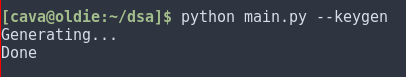
\includegraphics[scale=0.7]{keygen1.png}
  \centering
\end{figure}
\begin{figure}[h]
  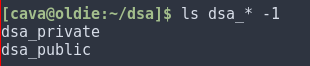
\includegraphics[scale=0.7]{keygen2.png}
  \centering
\end{figure}

\subsection{Podpisywanie wiadomości}
\begin{figure}[h]
  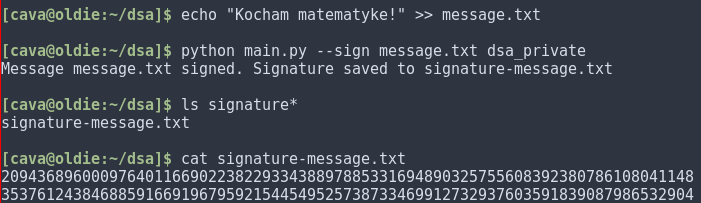
\includegraphics[scale=0.6]{sign.png}
  \centering
\end{figure}

\subsection{Weryfikacja podpisu}
\begin{figure}[H]
  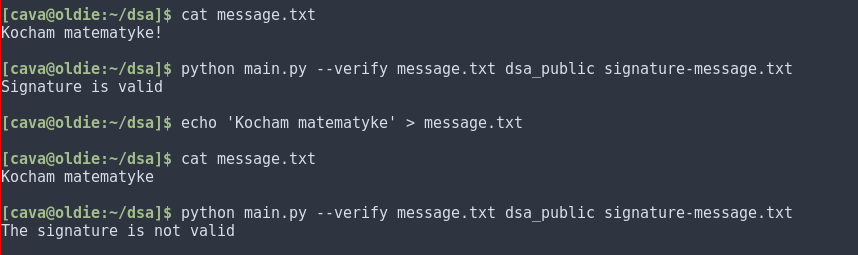
\includegraphics[scale=0.5]{verification.png}
  \centering
\end{figure}

\end{document}
